\begin{boxM}
    همانند سوال ۱ اسکریپت‌های توابع امتیازدهی به اسناد را می‌نویسیم.
\end{boxM}


\begin{figure}[h]
    \centering
    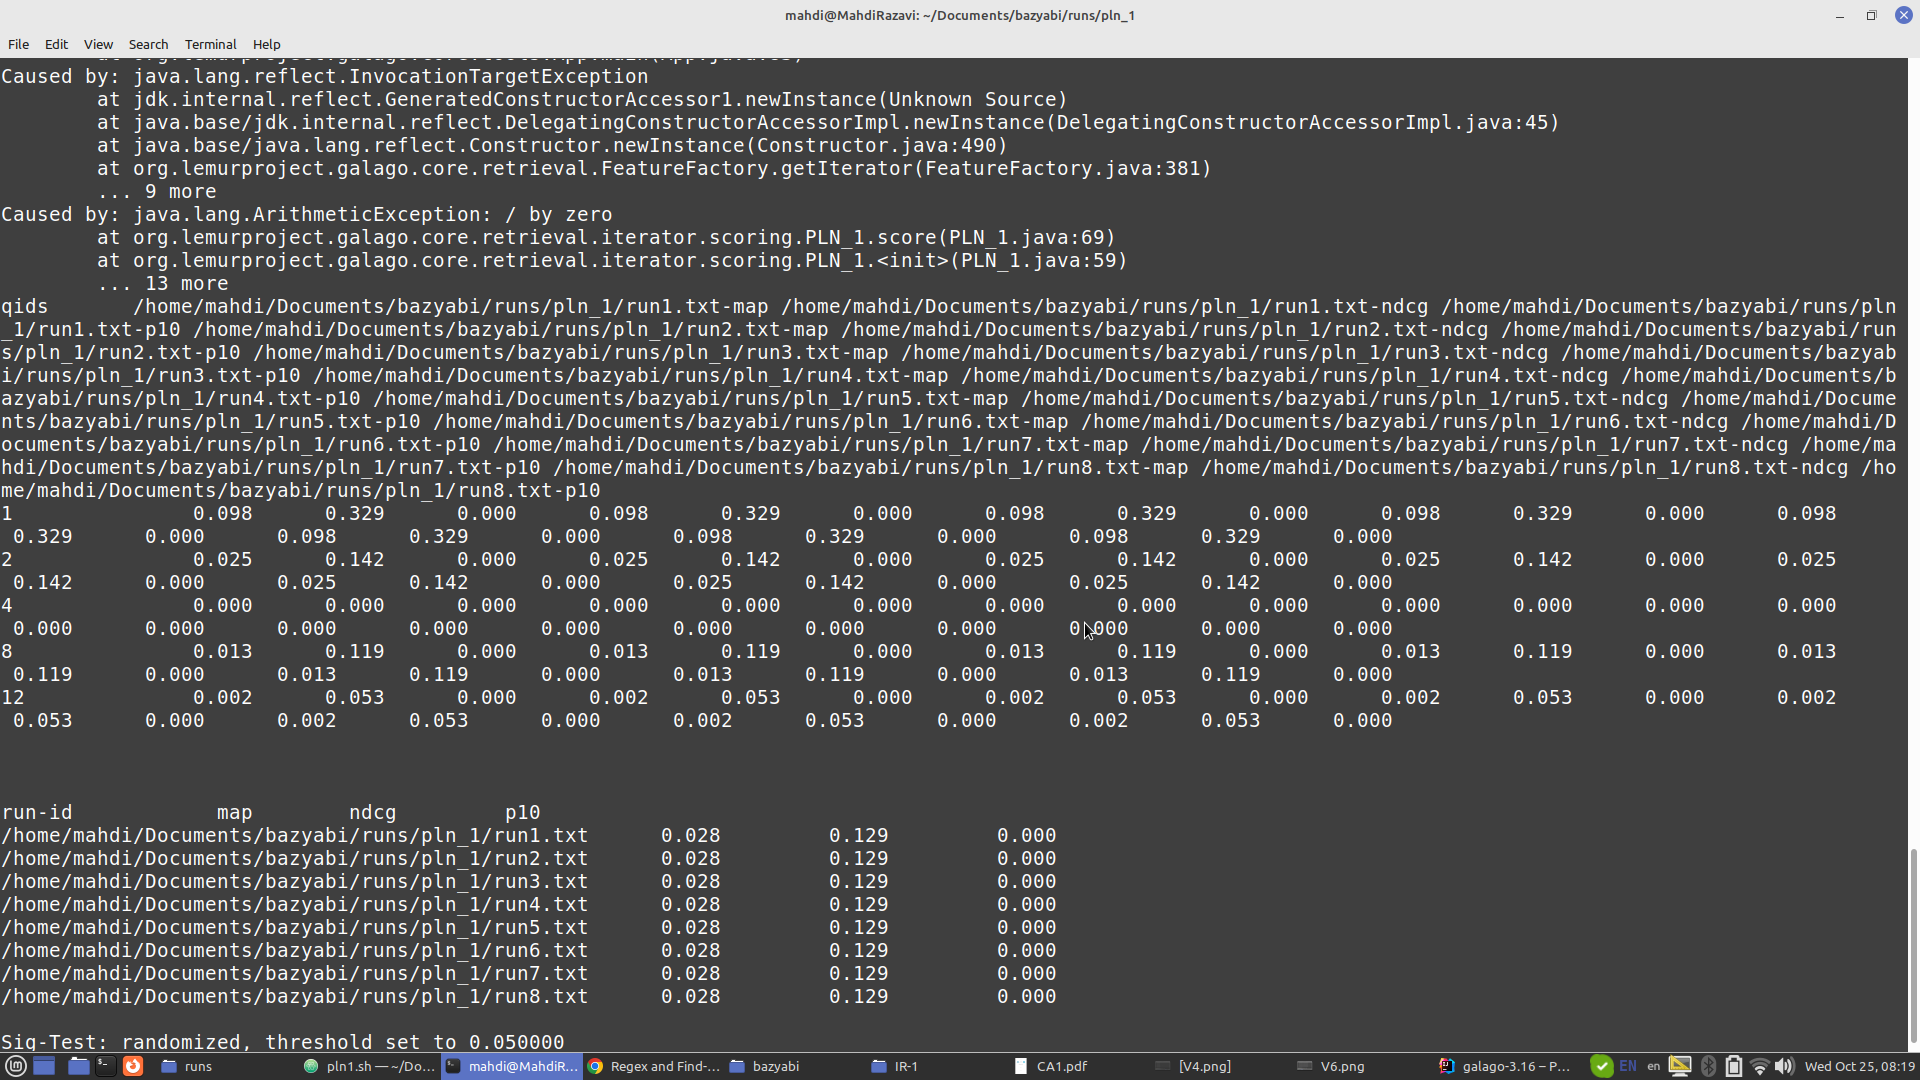
\includegraphics[width=0.8\textwidth]{IR1/images/pln_1.png}
    \caption{تاثیر تابع تبدیل ۱}
    % \caption{نتایج مرتب‌سازی با تابع امتیازدهی ۴}
    \label{fig:enter-label}
\end{figure}

\begin{boxM}
    متاسفانه تغییری در نتایج آزمایش‌ها مشاهده نشد.
    چون که آزمایش‌ها مستقل از
    \lr{k}
    می‌باشند ، 
    متوجه خواهیم شد که تاثیر پارامتر
    \lr{b}
    نیز بسیار ناچیز است.
\end{boxM}

\newpage

\begin{figure}[h]
    \centering
    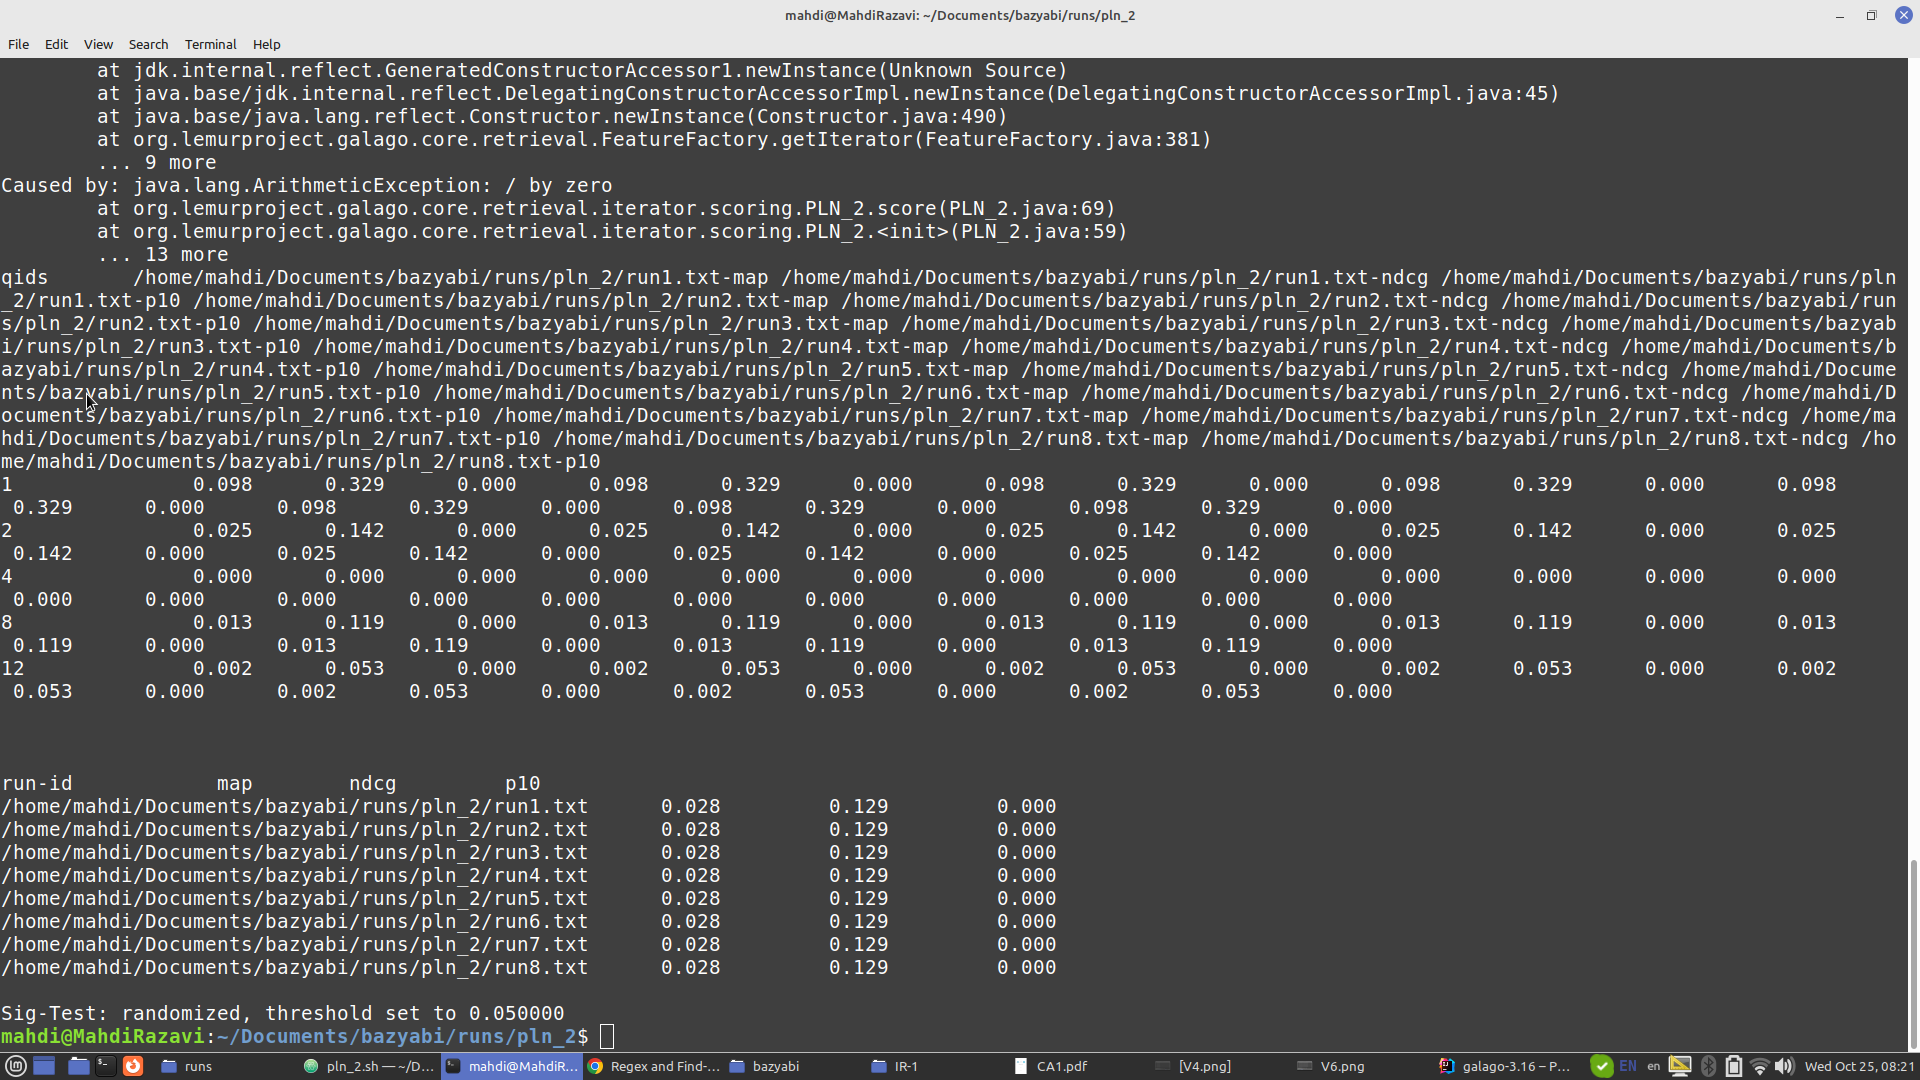
\includegraphics[width=0.8\textwidth]{IR1/images/pln_2.png}
    \caption{تاثیر تابع تبدیل ۲}
    \label{fig:enter-label}
\end{figure}

\begin{boxM}
    متاسفانه تغییری در نتایج آزمایش‌ها مشاهده نشد.
    چون که آزمایش‌ها مستقل از
    \lr{k}
    می‌باشند ، 
    متوجه خواهیم شد که تاثیر پارامتر
    \lr{b}
    نیز بسیار ناچیز است.
\end{boxM}